%! TEX ROOT = ./main.tex

\section{Experimental Evaluation}\label{sec:experiments}
%\MS{List the specifications of the cluster machine/laptop with which we have run our experiments.}
We evaluate a prototype implementation of Algorithm~\ref{alg:abcd-for-tracking}
on two examples. 
The design of nominal controller has been performed on a laptop with core i7-4510u CPU at 3.10GHz, with 8GB of
RAM.
The formal controller synthesis has been performed
on a cluster with 4 Intel Xeon E7-8857 v2 CPUs (48 cores in total) at 3GHz, with 1.5TB of
RAM.
\subsection{Inverted Pendulum}\label{subsec:invpend}
As a simple example, consider the standard problem of designing a controller for a frictionless inverted pendulum.
The goal of the controller is to bring the pendulum to vertical position while satisfying hard constraints on the state variables and control inputs.
A model of the system can be constructed using physical principles. Taking angular position ($\theta$) and angular speed ($r$) as state variables, the state vector is represented as $x=[\theta;r]^\top$ and its dynamics is described as $\dot x(t)=f_{ip}(x(t),u(t))+w(t)$, where $u(t)$ and $w(t)=[w_1(t);w_2(t)]^\top$ denote respectively the input torque and the disturbance, at time $t$ and
\begin{equation}\label{eq:inv_pend_ss}
	f_{ip}(x(t),u(t))=\begin{bmatrix}r(t)\\\frac{g}{L}sin(\theta(t))+u(t)\end{bmatrix}.
\end{equation}
%\begin{align*}\label{eq:inv_pend_ss}
%\dot\theta(t)&=r(t)+w_1(t)\nonumber\\
%\dotr(t)&=\frac{g}{L}sin(\theta(t))+u(t)+w_2(t)
%\end{align*}
%bounded with a polyhedral set $w(t)\in W$ for $W\subset\reals^2$, captures the modeling errors. 
The parameter $g=9.81 [m/s^2]$ is the gravitational acceleration
and $L$ is the length of the bar. 

Starting from initial state $x_0^{nom}=[-\pi;0]$, the control goal is to converge to an $\varepsilon-$neighbourhood of the equilibrium point 
$x_e=[0;0]^\top$. To this end, we first consider the undisturbed system ($W=\{[0;0]^\top\}$)  and use ALTRO (\MS{\cite{??}}) to generate a (nominal) trajectory $(x_0^\nom,\ldots,x_K^\nom)$ such that $x_K^{nom}\approx x_e$. Setting the sample time $\tau=0.05[sec]$, $L=9.81[m]$ and $K=100$, generating the nominal trajectory takes 0.14 seconds. Next, we use SCOTS in order to synthesize a controller such that the nominal trajectory is not violated beyond the specified tube around it under different levels of disturbance. Taking state space $X=[-\pi,\pi]\times[-2,2]$, input space $U=[-5,5]$, state space discretization step $\eta_s=[0.01;0.01]^\top$ and input space discretization step $\eta_i=0.2$, we use Algorithm~\ref{alg:abcd-for-tracking} to compute controllers for various $W$ and $\varepsilon$. Note that the full state space has $252229$ states. Table~\ref{tab:inv_pend} demonstrates the effect of tube width on the size of reduced state space and magnitude of disturbance under which SCOTS is able to find controller. It can be observed that by increasing the tube width, SCOTS is able to synthesize a controller for larger disturbance levels in the cost of increasing size of state space. Figure~\ref{fig:invpend_traj} demonstrates trajectories of the inverted pendulum system governed by controllers synthesized by ALTRO and SCOTS under appliance of constant disturbance vector $w=[0.111;0.111]^\top$. As expected, the controller designed by ALTRO is not able to keep the trajectory of the system within the tube around the nominal trajectory, whereas using the controller generated by SCOTS, the trajectory remains within the specified tube.
%Additionally, we require the state constraints $\theta_k\in[-\pi,\pi]$ and $v_k\in[-\pi/8,\pi/8]$ to hold at all time instances.
%\begin{figure}\label{fig:inv_pend}
%	\includegraphics[]{}
%	\caption{Variations of disturbance limit for which SCOTS is able to find a controller with tube size}
%\end{figure}
\begin{figure}\label{fig:invpend_traj}
	\centering
	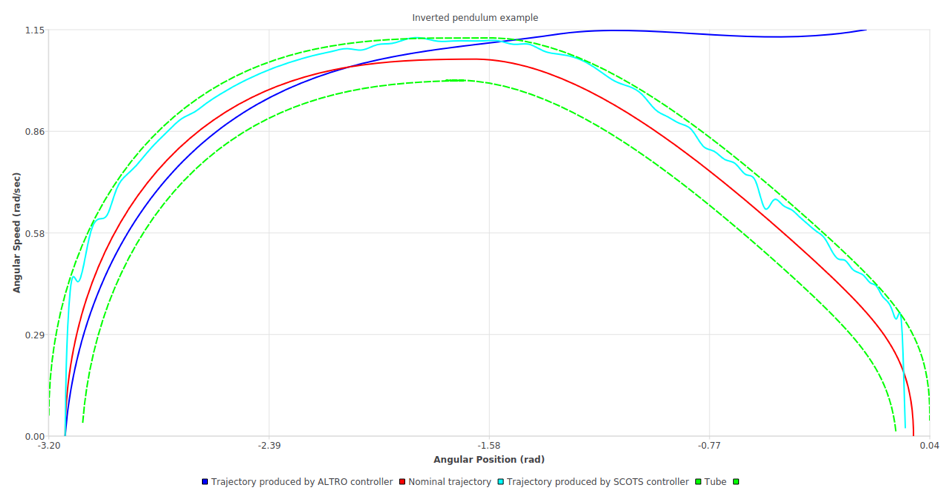
\includegraphics[width=0.85\textwidth]{traj_inv_pend.png}
	\caption{Trajectories of inverted pendulum when open loop controller produced by ALTRO and formally synthesized controller produced by (modified) SCOTS were used.}
\end{figure}
\begin{table}[h!]
	\centering
	\caption{Variations in $W$ (disturbance bounds under which using Algorithm~\ref{alg:abcd-for-tracking} a controller can be synthesized), size of state space and abstraction time (in seconds) for different tube width ($\varepsilon$).}
	\vspace{1mm}
	\begin{tabular}{|c|c|c|c|c|}
		\hline
		$\varepsilon$ &  $W$  & State space size size & Abstraction time ([sec])  \\
		\hline
		$\varepsilon<0.03$  & -    & -  & -  \\
		\hline
		0.03   & $[-0.032,0.032]^2$    & 3161  & 0.18  \\
		\hline
		0.05   & $[-0.077,0.077]^2$   & 5350  & 0.31  \\
		\hline
		0.07    & $[-0.116,0.116]^2$  & 7557  & 0.46  \\
		\hline
		0.1  &  $[-0.116,0.116]^2$   & 10965  & 0.66  \\
		\hline
		0.12    & $[-0.116,0.116]^2$  & 13258  & 0.80  \\
		\hline
		0.15   &$[-0.116,0.116]^2$  & 16743     & 1.014 \\
		\hline
	\end{tabular}
	\label{tab:inv_pend}
\end{table}
\subsection{Ship Docking}\label{subsec:6dship}
Next, we consider controller synthesis for a ship docking scenario wherein a ship starts moving toward the dock from a certain distance and the control goal is hence to bring the ship from its start point into the dock such that the ship's speed near the dock is very small. To represent the ship's model in state space, we partition the state vector as $x=[\eta;\nu]$, where $\eta=[N;E;\psi]^\top$ are the South-North and West-East positions and heading of the ship, $\nu = [u ;v ;r]^\top$ are the surge and sway velocities, and yaw rate of the ship. Moreover the disturbance vector is partitioned as $w=[w_c;w_{wind}]^\top$ where $w_c\in\reals^3$ is the disturbance due to the current velocities and $w_{wind}\in\reals^3$ is the disturbance corresponding to wind forces. One can write the ship dynamics as $\dot x(t)=f_s(x(t),u(t))+\bar w(t)$, where $u\in\reals^3$ and $\bar w=[w_c;M^{-1}R(\psi)^{\top}w_{wind}]^\top$ denote the control input vector and transformed disturbance and
\begin{equation}\label{eq:ship_ss}
f_{s}(x(t),u(t))=\begin{bmatrix}R(\psi)\nu\\M^{-1}(u(t)-C(\nu)\nu-D\nu)\end{bmatrix}.
\end{equation}
%The state space equations of the ship model are
%\begin{align*}
%&\dot{\eta}=R(\psi)\nu+w_c \\
%&M\dot{\nu}+C(\nu)\nu+D\nu=u+R(\psi)^{\top}w_{wind},
%\end{align*}
where $R=R(\psi)=\begin{bmatrix}
cos(\psi) &-sin(\psi) &0\\
sin(\psi) & cos(\psi) & 0\\
0 & 0 & 1
\end{bmatrix}$ is a rotation matrix. Further, the inertia matrix $M=\begin{bmatrix}
87.4 & 0 & 0 \\
0 & 98.3 & 2.48 \\
0 & 2.48 & 22.2
\end{bmatrix}$, the damping matrix $D=\begin{bmatrix}
6.58 & 0 & 0 \\
0 & 37.7 & 2.66 \\
0 & 2.66 & 19.3
\end{bmatrix}$ and Coriolis matrix $C(v)=\nu(1)\begin{bmatrix}
0 & 0 & 0 \\
0 & 0 & 98.3 \\
0 & 0 & 2.48
\end{bmatrix}$ are chosen for a $1:30$ scale model of a platform supply vessel.

Starting from an initial state $x_0^{nom}=[0;0;0;0;0;0]^\top$, the control goal is to converge to $\varepsilon-$neighbourhood of the point 
$x_d=[1;1;0;0;0;0]^\top$. To this end, we first consider the undisturbed system and use ALTRO to generate a (nominal) trajectory $(x_0^\nom,\ldots,x_K^\nom)$ such that $x_K^{nom}\approx x_d$. Setting the time step $\tau=3[sec]$, and $K=8$, generating the nominal trajectory takes around 3.16 seconds. Next, we use SCOTS in order to synthesize a controller such that the nominal trajectory is not violated beyond the specified $\varepsilon$, under different levels of disturbance. Taking state space $X=[-.3,1.25]^2\times[-.3,.7]\times[-.03,.12]\times[-.03,.075]\times[-.085,.095]$, input space $U=[-2,2]^3$, state space discretization step $\eta_s=[.05;.05;.05;.005;.005;.005]^\top$ and input space discretization step $\eta_i=[.5;.5;.5]^\top$, we used Algorithm~\ref{alg:abcd-for-tracking} to compute controllers for $\varepsilon=2\eta_s$ and $W=[-.001;.001]^3\times[-.0001,.0001]^3$. Note that size of state space is decreased from $542631936$ into $4569816$ while abstraction and synthesis take $1539.28$ and $413.726$ seconds, respectively.
 %Figure~\ref{fig:inv_pend} demonstrates variations of disturbance limit under which SCOTS is able to find a controller for different tube width. %It can be observed that by increasing the tube width, SCOTS is able to synthesize a controller for larger disturbance levels. Figure~\ref{fig:invpend_traj} demonstartes trajectories of the system  \eqref{eq:inv_pend_ssq} governed by controllers synthesized by ALTRO and SCOTS under appliance of constant disturbance vector \MS{$[??,??]$}. As expected, the controller designed by ALTRO is not able to tackle disturbance, while using the controller generated by SCOTS, the trajectory remains within the desired bound.

%\begin{figure}\label{fig:inv_pend}
%	\includegraphics[]{}
%	\caption{Variations of disturbance limit for which SCOTS is able to find a controller with tube size}
%\end{figure}
%\begin{figure}\label{fig:invpend_traj}
%	\includegraphics[]{}
%	\caption{}
%\end{figure}




